%!TEX root = thesis.tex

% a related work section in which the relevant literature is presented and linked to the project;
% ~15 pages 

\chapter{Related work}
\label{chap:rw}
A number of research topics are relevant for this thesis: how to use existing standards for publishing sensor data to the semantic web, developing ontologies that are suitable for many different kinds of sensor data and how to aggregate sensor data based on geographical features and time. This chapter discusses the recent relevant literature on these topics. However, first it will introduce the \acl{swe} suite of standards and the semantic web.  

\section{Sensor Web Enablement}

\cite{SW:OGC} present \acf{swe}, which is a suite of standards developed by \ac{ogc}. It contains two parts: the information model and the service model. The information model includes \ac{om}, \ac{sensorml} and \ac{swe} common. \ac{om} defines the data model and encoding for observation data  and \ac{sensorml} defines the data model and encoding for sensor metadata. \ac{swe} common is a low-level data model for exchanging sensor related data. The service model contains the \ac{sos}, \ac{sps}, \ac{sas} and \ac{wns}. A \ac{sos} can be used to retrieve observation data, a \ac{sps} to plan actions of a sensor, and a \ac{sas} to receive alerts about subscribed events. With a \ac{wns} users can have asynchronous dialogues (message interchanges) with one or more other services. Recently the SensorThings \ac{api} has been added to the list of \ac{swe} services (see \url{http://ogc-iot.github.io/ogc-iot-api/index.html}). The SensorThings \ac{api} is a service for retrieving observation data and sensor metadata for \ac{iot} applications. This thesis focusses on \ac{om}, \ac{sensorml} and \ac{sos}. The following paragraphs will therefore described these standards in more detail.

\subsection{Observation and Measurements}

\begin{figure}
	\centering
	\includegraphics[width=0.8\linewidth]{UML/OM_Observation.png}
	\caption{Basic observation in the \ac{om} data model \citep[p. 9]{SW:ISO}}
	\label{fig:OM_observation}
\end{figure}

In the \acf{om} data model an observation is modelled using a number of concepts. First of all, there is a feature of which sensor data is wanted. This is the so-called \acf{foi}. This feature has a property that can be observed, also known as an observable property. For example, the air at a certain location (\ac{foi}) has a certain temperature (observable property). A \ac{foi} can also be a geographical feature such as a river or a forest area. \ac{om} uses the concept of \ac{foi} rather than the sensor location, because for some observations the exact location may not be trivially available. Furthermore, specific specimens are in some cases removed from their sampling location and observed at another location afterwards. This would create problems when defining a location of observation, hence the use of \aclp{foi} in the \ac{om} data model. An observation is defined as the \enquote{act of measuring or otherwise determining the value of a property} \citep[p. 3]{SW:ISO}. The observation uses a procedure, which is a method, algorithm or instrument, or system of these. A procedure can therefore be a sensor, an algorithm processing the raw observation data and/or a system of sensors observing a property of the \ac{foi}. The output of the procedure is a result. The result consists of a value and a corresponding \acf{uom}. For example: 15 (value) degrees Celcius (\ac{uom}). 

A procedure can produce many results about the same \ac{foi} over time. Therefore, three temporal concepts have been modelled: result time, phenomenon time and valid time. The result time is the timestamp of the observation result, or in other words: the moment the observation result became available. It is not necessarily the time that corresponds to the phenomenon, depending on when the observation procedure is performed (specimens can be taken from a sampling location and observed later) and the amount of time it takes to perform a procedure. Therefore, the phenomenon time describes the time that the observation applies to the property of the \ac{foi}. The valid time is a time range that indicates when an observation is a valid indication of the property of the \ac{foi}. When observing glacier motion at a speed of several  meters per year an observation result might be valid for a day. On the other hand, observations with large fluctuations during the day might only be valid for a number of minutes up to an hour. This is the case for example with air quality observations in cities, that have large fluctuations with peaks during the rush hours.     

Additional metadata about an observation can be added using the metadata class in the data model. To provide context about an observation the `related observations' class has been added to the \ac{om} model as well. Figure \ref{fig:OM_observation} shows the \ac{uml} diagram containing the different concepts explained in this paragraph and the relations between them.  

\subsection{SensorML}

The \acf{sensorml} aims to \enquote{provide a robust and semantically-tied means of defining processes and processing components associated with the measurement and post-measurement transformation of observations} \citep[p. ix]{SW:OGC7}. Creating interoperability at the syntactic and semantic level allows processes to be better understood by machines, utilized automatically in complex workflows, and to be easily shared between intelligent sensor web nodes. \ac{sensorml} is a framework that can be used to define the geometric, dynamic, and observational characteristics of sensors and sensor systems in order to achieve syntactic and semantic interoperability. 

\begin{figure}
	\centering
	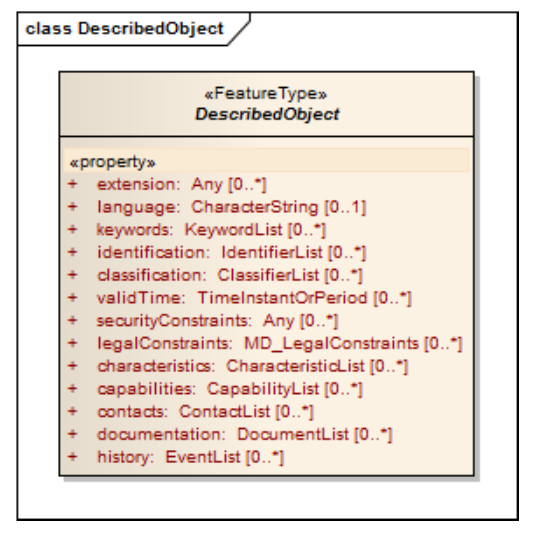
\includegraphics[width=0.5\linewidth]{UML/describedObject.png}
	\caption{`DescribedObject' class in \ac{sensorml} \citep[p. 39]{SW:OGC7}}
	\label{fig:describedObject}
\end{figure}

In \ac{sensorml} there is a destinction between two types of processes: physical and non-physical processes. For a physical process information about the spatio-temporal position is important. This is the case with for example detectors, actuators, and sensor systems. Non-physical processes are mathematical operations or functions. A process is modelled as a specialisation of the `DescribedObject' class. This class provides a set of metadata which are useful for all process classes in \ac{sensorml}. Figure \ref{fig:describedObject} shows the properties of a described object class instance. The `AbstractProcess' class is derived from the described object and includes the properties: inputs, outputs, parameters, typeOf, featureOfInterest, configuration and modes. This forms the basis for defining both physical and non-physical processes. The `AbstractPhysicalProcess'  class is derived from the describe object class and adds spatial and temporal coordinates for the physical process device. The final step in defining a physical process is to specialise the abstract physical process with the `PhysicalComponent' class. The physical component describes the device that provides a processing function. Figure \ref{fig:physicalProcess} shows the \ac{uml} class diagram of a physical process. 

\begin{figure}
	\centering
	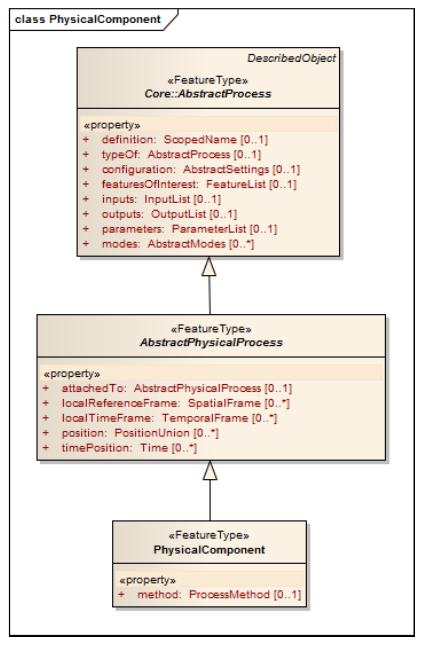
\includegraphics[width=0.6\linewidth]{UML/physicalProcess.png}
	\caption{Definition of a physical process in \ac{sensorml} \citep[p. 57]{SW:OGC7}}
	\label{fig:physicalProcess}
\end{figure}

Although \ac{sensorml} is not dependent on \ac{om} the result of a process modelled by \ac{sensorml} is typically considered as an observation result. This is the case if it is measuring a physical property or phenomenon. Therefore, the output values described in \ac{sensorml} and resulting from a sensor or process may be encoded as an \ac{om} Observation. Inversely, the procedure property of an \ac{om} Observation instance can be described using SensorML \citep{SW:OGC7}.

\subsection{Sensor Observation Service}
\label{par:sos}
\begin{sloppypar}
	There are three core requests that can be made to retrieve sensor (meta)data from a \ac{sos}: \texttt{GetCapabilities}, \texttt{DescribeSensor} and \texttt{GetObservation}. \texttt{Get} \texttt{Capabilities} returns a complete overview of what the \ac{sos} has to offer. The \texttt{DescribeSensor} request returns detailed information about individual sensors. These three core requests are mandatory in a \ac{sos} under the 2.0 specifications \citep{SW:OGC2}. There are also a number of optional extensions to a \ac{sos}: \texttt{GetFeatureOfInterest}, \texttt{GetObservationById}, \texttt{InsertCapabilities}, \texttt{InsertObservation}, \texttt{InsertSensor}, \text{DeleteSensor}, \texttt{InsertResult}, \texttt{InsertResultTemplate} and \texttt{GetResultTemplate}. Requests can be made as a \ac{http} GET request or a \ac{http} POST request. There can be different response formats, but there is always at least the option to retrieve the response as an \ac{xml} document. Based on the specification by \cite{SW:OGC2} the following paragraphs describe the core and optional requests of a \ac{sos}, as well as the structure of their responses. 
\end{sloppypar}

\subsubsection{Get capabilities}
\label{par:capabilities}
The \texttt{GetCapabilities} request is the first step in communicating with a \ac{sos}. The request is made by taking the \ac{http} address of the \ac{sos} and adding \url{service=SOS\&request=GetCapabilities}. It returns a document including information on what the service has to offer. The document contains a number of sections: service identification, service provider, operations metadata, filter capabilities and contents. 

In the service identification section there is general information about the service, such as the title and supported \ac{sos} versions, but also whether there are fees or access constraints. The service provider section contains details on which organisation provides the \ac{sos} and lists their contact information. The operations metadata section lists the supported request types. It also contains an overview of all features-of-interest, observed properties, procedures and offerings. Offerings are similar to layers in a \ac{wms}, grouping together observations collected by one procedure.

The contents section describes the data that can be retrieved, grouped in offerings. Each offering has an identifier, together with information on the procedure, observable properties and the feature-of-interest type. Which filters can be applied in a request is described in the filter capabilities section. The supported parameters for both spatial and temporal filters are listed here.

\begin{figure}
	\centering
	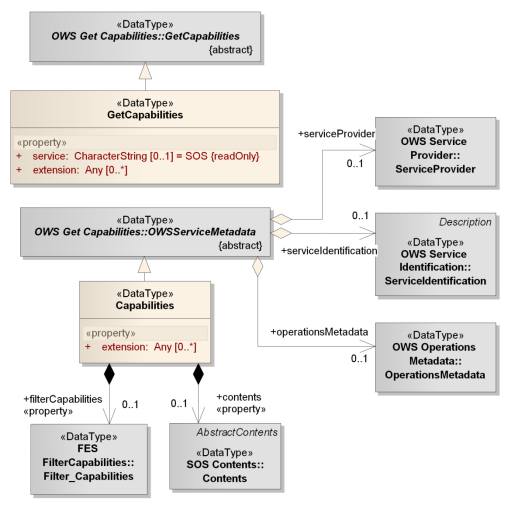
\includegraphics[width=0.7\linewidth]{figs/SOS_2_dataModel_GetCapabilities.PNG}
	\caption{Data model behind the capabilities document of a \ac{sos} \citep{SW:OGC2}}
	\label{fig:Capabilities}
\end{figure}

\subsubsection{Describe sensor}

\begin{sloppypar}
	The \texttt{DescribeSensor} request gives detailed information on a specific sensor. The request is built by taking the \ac{http} address of the \ac{sos} and adding \url{service=SOS\&version=2.0.0\&request=DescribeSensor\&procedure=aprocedure\&proceduredescriptionformat=aformat} where the procedure and procedure description format have to contain values defined in the capabilities document.
\end{sloppypar}

% write about SWE describesensor schema
% http://www.opengis.net/swes/2.0
% http://schemas.opengis.net/swes/2.0/swesContents.xsd

\subsubsection{Get observation}
\label{par:getObservation}

Using \texttt{GetObservation} actual measurements can be retrieved. The request is made by taking the \ac{http} address of the \ac{sos} and adding \url{service=SOS\&version=2.0.0\&request=GetObservation}. This returns a response with the default parameters, which can differ from one \ac{sos} to another. To further specify the request, paramaters can be added such as: observed property, procedure, feature-of-interest, offering and outputformat. Spatial and temporal filters can be added if these are supported by the service. 

The \texttt{GetObservationByID} request is an extension that let's users retrieve an observation using an identifier that points to a certain observation. 

% write about OM observation schema


\subsubsection{Get feature of interest}
The \texttt{GetFeatureOfInterest} request allows to retrieve information about the feature of interest of a certain observation. The response can be all features of interest or only ones that are related to a specific observed property, procedure or spatial filter. This request also allows logical operators, for example: \enquote{GetFeatureOfInterest ( observedProperty := temperature AND procedure := thermometerX OR anemometerY )} \citep[p. 40]{SW:OGC2}. The response is a document with `GFI\_features' (\ac{iso} 19109) \citep{GEO:ISO}, which are implemented in the \ac{gml} (\ac{iso} 19136) \citep{GEO:ISO2} by the element gml:AbstractFeature and type gml:AbstractFeatureType \citep[p. 38]{SW:ISO}.

\subsubsection{Transactional extensions}
\begin{sloppypar}
It is possible to update the content of a \ac{sos} using transactional request. There are six of these requests that could be implemented: \texttt{InsertCapabilities}, \texttt{InsertObservation}, \texttt{InsertSensor}, \text{DeleteSensor}, \texttt{InsertResultTemplate} and \texttt{InsertResult}. \texttt{InsertCapabilities} allows a request to add data to the capabilities document described in Paragraph \ref{par:capabilities}. The request contains three mandatory parameters and one optional parameter: it is required to have the \texttt{procedureDescriptionFormat}, \texttt{FeatureOfInterestType} and \texttt{ObservationType}. Optionally, \texttt{SupportedEncoding} could be added to the request. An \texttt{InsertCapabilities} should be made in combination with a \texttt{InsertObservation}, \texttt{InsertSensor} or \texttt{InsertResult} request.
\end{sloppypar}

A \texttt{InsertResultTemplate} request allows to upload a template for result values. It should contain data about the offering, the observation template, the result structure and result encoding. The actual results can be added later using an \texttt{InsertResult} request. This request is different from the \texttt{InsertObservation} request, as it only inserts the result value of an observation, assuming that the metadata is already present in the \ac{sos}. This is useful when there is limited communication bandwidth and processing power. This request has two mandatory parameters: a pointer to the template and the observation value to be inserted. An \texttt{InsertObservation} request allows observations to be added to a registered sensor system. It also has two mandatory parameters: a pointer to an offering and the observation to be inserted.

Individual sensors can be inserted or deleted using \texttt{InsertSensor} and \texttt{DeleteSensor} requests. For inserting a sensor the following parameters are required: the procedure description format, a procedure description, the observable property, a feature of interest type and an observation type. For deleting a sensor an identifier that points to a specific sensor needs to be passed as a parameter.


\section{Semantic web}
The semantic web is an extension of the internet using standards by the \ac{w3c}. Figure \ref{fig:SemanticWeb} shows the hierarchy of data on the semantic web, starting with \acp{uri} at the bottom which are pointers to parts of data. Their actual content is made available in self describing documents. In these documents concepts are defined using existing ontologies. The top layers of the pyramid (logic, proof and trust) have not yet been standardized, and are still a topic of research.  

The semantic web is based on the open world assumption. This means is that \enquote{the thruth of a statement is independent of whether it is known} \citep[p. 103]{LD:Hebeler}. Traditional software application use the closed world assumption. Here a statement is assumed false if the answer is unknown. A simple example of this is a database table containing costumers of a store. If a person's name is not in that table the closed world assumption decides that this person is not a costumer of the store. The name is unknown and hence the statement `he/she is a customer' is false. An open world assumption would decide that it is simply unknown whether this person is a costumer, since it hasn't been described anywhere. The closed world assumption only works in an environment where all information is complete. There should be no possibility in our example that people who are customers are not present in the database table). The case of the internet is that there is an enormous collection of data stored in different places and it can never be guaranteed that this data is complete. Therefore the semantic web is based on the open world assumption \citep{LD:Hebeler}. 

In the next paragraphs the framework of the semantic web --  the \acf{rdf} -- will be described, followed by different \ac{rdf} notations. The last part explains the concept of \acp{purl}.

\begin{figure}[!h]
	\centering
	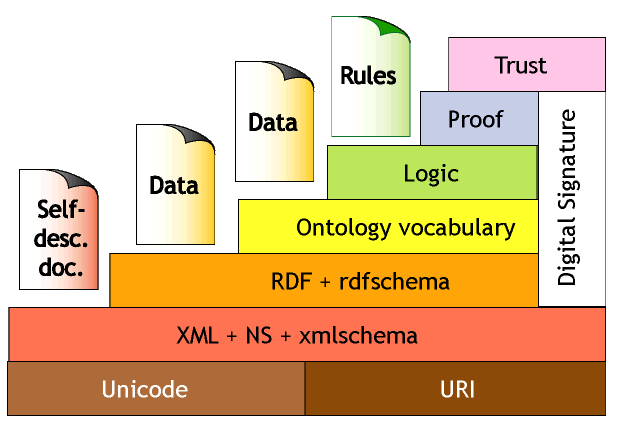
\includegraphics[width=0.7\linewidth]{figs/semanticweb2.png}
	\caption{Hierarchy of the semantic web \protect\footnotemark}
	\label{fig:SemanticWeb}
\end{figure}

\subsection{Resource Description Framework}
In \ac{rdf} data is stored as so-called `triples'. These triples are structured as: subject, predicate and object \citep{LD:Berners-lee}. The subject and the object are things and the predicate is the relation between these two things. For example, to define a geographic feature such as the municipality of Delft on the semantic web a number of triples can be made. Figure \ref{fig:Triples} shows how Delft can be defined as a municipality with a certain geometry using triples of subject, predicate and object.

\begin{figure}
	\centering
	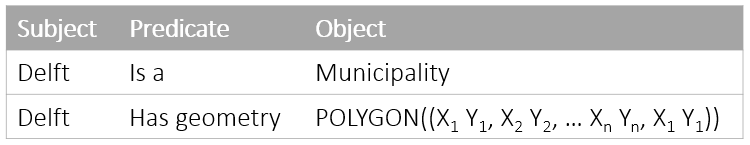
\includegraphics[width=0.7\linewidth]{figs/Triples.png}
	\caption{Triples of object, predicate and subject define Delft as a municipality with a geometry}
	\label{fig:Triples}
\end{figure}

Three types of data can make up these triples \citep{LD:W3C6}. The first type is an \ac{iri}. This is a reference to a resource and can be used for all positions of the triple. A \ac{url} is an example of an \ac{iri}, but \ac{iri}s can also refer to resources without stating a location or how it can be accessed. An \ac{iri} is a generalisation of an \ac{uri}, and also allows non-ASCII characters. In the example of the municipality of Delft, \ac{iri}s can be used to define `Delft' and `Municipality', but also for the predicates `is a' and `has geometry'. The second type of data is a literal. A literal is a value which is not an \ac{iri}, such as strings, numbers or dates. These values can only be used as object in a triple. In the example of Delft, a literal could be used to store the actual geometry of the boundary: POLYGON(( $x_{1},y_{1}$ $x_{2},y_{2}$ ... $x_{n},y_{n}$, $x_{1},y_{1}$ )). A literal value can have a datatype specification \citep{LD:W3C7}. This is added to the literal with the \^{}\^{} symbols, followed by the \ac{iri} of the datatype specification. In Figure \ref{fig:Turtle} the datatype is `geo:wktLiteral'.

Sometimes it is useful to refer to things without assigning them with a global identifier. The third type is the blank node and can be used as an subject or object without using an \ac{iri} or literal \citep{LD:W3C6}.  

\footnotetext{{from \url{https://www.w3.org/2000/Talks/1206-xml2k-tbl/slide10-0.html}} by Tim Berners-Lee}

\subsection{Notation}
There are a number of different notations for writing down these triples (serialisation), such as \ac{xml} \citep{LD:W3C3}, N3 \citep{LD:W3C5} and Turtle \citep{LD:W3C4}. Turtle will be used in this thesis, because it is commonly used notation which is also relatively easy to read for humans. The DBPedia \ac{iri} is used for the object `Municipality'. The `is a' predicate is represented by a built-in \ac{rdf} predicate which can be written simple as `a'. The second predicate is `hasGeometry' for which the GeoSPARQL \ac{iri} is used. The geometry is a literal in the \ac{wkt} format. Note that the subject is only written once when there are multiple triples with the same subject. Triples that share the same subject are divided by semicolons. A point marks the end of the last triple with a specific subject.

\begin{figure}
	\centering
	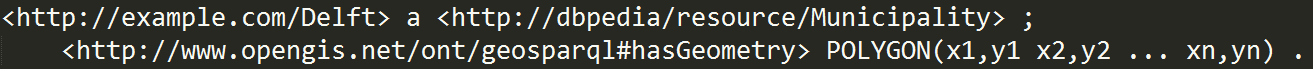
\includegraphics[width=1\linewidth]{figs/Turtle.png}
	\caption{Triples of Figure \ref{fig:Triples} in the Turtle notation}
	\label{fig:Turtle}
\end{figure} 

\subsection{Persistent Uniform Resource Locators}
\acp{url} are an essential part of the web. However, if an \ac{url} changes the existing links towards this \ac{url} are broken. To prevent this \acp{purl} are being used. A \acl{purl} is a \enquote{naming and resolution service for general Internet resources} \citep{LD:PURL}. This allows organisations to change the location of their data without changing the \ac{url} to which can be linked. A \ac{purl} server receives the \ac{url} and redirects the client to the current location of the resource. If the location of the resource 
changes, the server can be informed. It will then redirect clients to the new location (Figure \ref{fig:PURL}).  

\begin{figure}
	\centering
	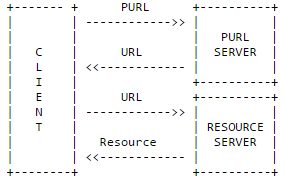
\includegraphics[width=0.6\linewidth]{figs/purl.png}
	\caption{Persistent Uniform Resource Locator (PURL) resolves to the current resource location \citep{LD:PURL}}
	\label{fig:PURL}
\end{figure} 


%\begin{figure}
%	\centering
%	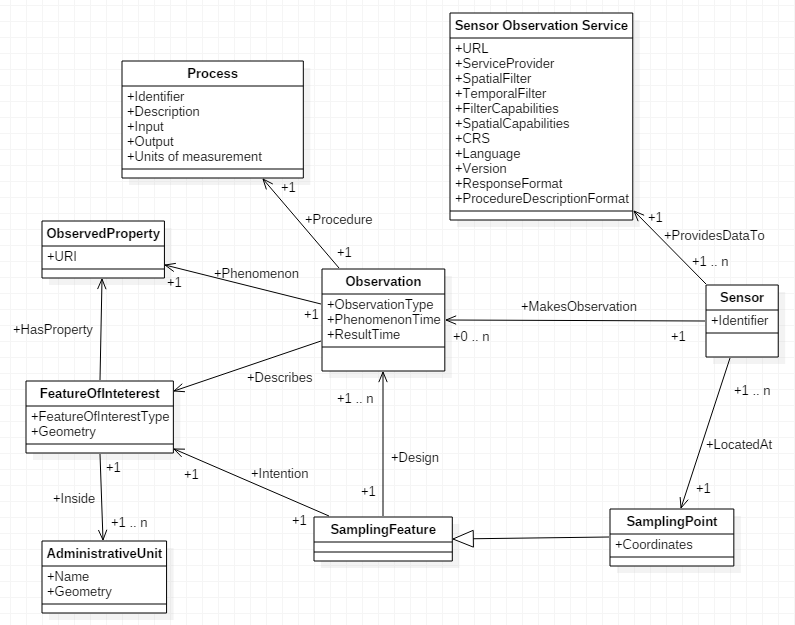
\includegraphics[width=1\linewidth]{UML/UML_Diagram.png}
%	\caption{\ac{uml} diagram of sensor observations service, based on \cite{SSW:Cox3} and \cite{SDI:INSPIRE2}}
%	\label{fig:UML}
%\end{figure}

%\section{Aggregation}
%There are many different ways to aggregate sensor data, for example by taking the minimum value, the maximum value, the average value, the sum, etc. Also, spatial aggregation techniques (based on neighbourhood analysis) can be considered to adjust for spatio-temporal irregularities as mentioned by \cite{SW:Ganesan}. In order to determine which method of aggregation is applicable for a specific kind of sensor data the sensor metadata will contain links to appropriate aggregation methods. However, which methods are appropriate should be based on expert knowledge.



\section{Sensor metadata in catalogue services}
The \ac{ogc} has developed a way of including sensors into a catalogue service using sensor registries. The different services related to this are described in this paragraph, starting with the \acf{csw}, after which the \acf{sor} and \acf{sir} services will be presented.

\begin{figure}
	\centering
	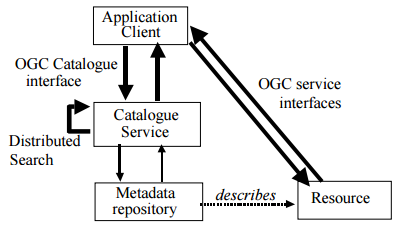
\includegraphics[width=0.6\linewidth]{UML/CSW.png}
	\caption{CSW model architecture \citep[p. 26]{GEO:OGC2}}
	\label{fig:CSW}
\end{figure}

\subsection{Catalog Service for the Web}
\label{par:CSW}
 The \ac{csw} is an \ac{ogc} standard for a geoweb service that contains \enquote{collections of descriptive information (metadata) for data, services, and related information objects} \citep[p. xiv]{GEO:OGC2}. Figure \ref{fig:CSW} shows the intermediary role of this service between client and data sources. It also shows that the \ac{csw} can use data from three different sources to return to a client: a local metadata repository, a resource service, or another \ac{csw}. The resource service can use an \ac{ogc} interface, but this is not required. 
 
 \begin{sloppypar}
 The \ac{csw} has the following requests for retrieving metadata: \texttt{GetCapabilities},  \texttt{DescribeRecord}, \texttt{GetDomain}, \texttt{GetRecords} and \texttt{GetRecordByID}. Metadata producers can use the \texttt{Transaction} and \texttt{Harvest} requests to respectively change or add content of a \ac{csw}. The \texttt{GetCapabilities} request returns a capabilities document to the client showing what the service has to offer. This request and response is required for all \ac{ogc} geoweb services and contains sections such as: service identification, service provider, operations metadata and filter capabilities. The service identification section lists general information about the service, such as the title and supported \ac{csw} versions, but also whether there are fees or access constraints. The service provider section contains details on which organisation provides the \ac{sos} and lists their contact information. The operations metadata section lists the supported request types. The filter capabilities show the different filters that are supported by the \ac{csw} instance. 
\end{sloppypar}

The \texttt{DescribeRecord} request allows the client to recieve a description of (a part of) the information model inside the catalog service. Parameters for namespaces or type names can be added to retrieve a part of the information model. The optional \texttt{GetDomain} request can be used to retrieve information about the range of values for a metadata record element or request parameter. A \texttt{GetRecords} request can be made to search for and retrieve catalogue records or to see if a they are present. The query element is the encoding for the search part of the \texttt{GetRecords}. The constraint parameter contains the query element and the constrain language parameter set the language that is being used to make the query. To see whether a record is present the outputSchema parameter and the `ElementName' or `ElementSetName' parameter(s) should be used. The \texttt{GetRecordsByID} request returns records using their identifier.

The \texttt{Transaction} request can be used to create, modify and delete catalogue records. \ac{http} GET requests using \ac{kvp} are not supported for this operation, because it is not a convenient way to encode the transaction payloads. Instead POST requests should be used exclusively for this. The transaction element in the request contains the type of action: insert, update and/or delete. 

\begin{figure}
	\centering
	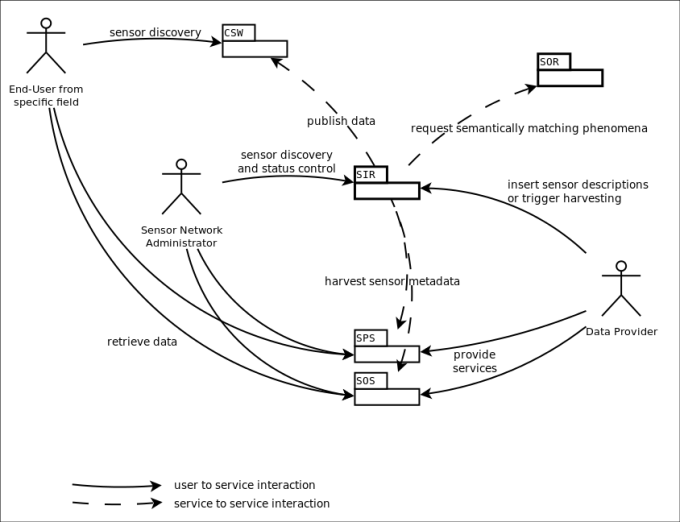
\includegraphics[width=0.8\linewidth]{figs/sor_sir.png}
	\caption{Overview of the interaction between CSW, SIR, SOR and potential users \citep{SW:52North2}}
	\label{fig:SorSir}
\end{figure}

\subsection{Sensor Observable Registry}
The \ac{sor} is \enquote{a web service interface for managing the definitions of phenomena measured by sensors as well as exploring semantic relationships between these phenomena} \cite[p. vi]{SW:OGC4}. This is a web service developed by \ac{ogc} to enable semantic reasoning on sensor networks, especially concerning phenomenon definitions. This should make it easier to discover sensors that observe a certain phenomenon and to interpret sensor data.

The \ac{sor} has four different requests: \texttt{GetCapabilities}, \texttt{GetDefinition-} \texttt{URNs}, \texttt{GetDefinition} and \texttt{GetMatchingDefinitions}. The \texttt{GetCapabilities} request provides an overview of what the \ac{sor} has to offer. The capabilities document that is returned to the client contains four sections. These sections are required for every \ac{ogc} geoweb service and the first three are the same as described in Paragraph \ref{par:CSW}. The fourth section is the content section. This part of the capabilities document contains the following information: the number of entries inside the \ac{sor} instance, keywords describing the content of the \ac{sor} instance, the application domain for which a specific \ac{sor} can be applied and an `ontologyRepositoryURL'. This \ac{url} points to a repository that contains an ontology used by this \ac{sor}.

\texttt{GetDefinitionURNs} returns a list of \acp{urn} identifying the definitions that are present in the \ac{sor}. Optionally a client can add a `SearchSensor' parameter to filter \acp{urn}. This parameter takes a substring that shall occur within the definition \acp{urn} to be returned. Also, a maximum limit for the amount of returned \acp{urn} can be added using the `maxNumberOfResults' parameter. The optional parameter `startResultElement' can be used to input the number of the first returned result element. For retrieving the definition of a specific \ac{urn} a \texttt{GetDefinition} request can be made. This request takes an \ac{urn} of the phenomenon for which a definition should be retrieved as input. The definition is returned as a \ac{gml} dictionary entry. 

\texttt{GetMatchingDefinitions} allows clients to retrieve definitions of observables which in some way are related to another given phenomenon. The relations `generalization', `specialization' and `equivalency' are currently supported for finding matching definitions \citep{SW:OGC4} and have to be specified in the request using the `matchingtype' parameter. This parameter can take one of three values: SUPER\_CLASS, EQUIVALENT\_CLASS or SUB\_CLASS. Additionally, the request can have the `searchDepth' parameter, which represents the maximum amount of steps that are allowed in case of a transitively related phenomena.  

\subsection{Sensor Instance Registry}
Another web service interface specification by \ac{ogc} is \ac{sir}. \ac{sir} is aimed at \enquote{managing the metadata and status information of sensors} \cite[p. xii]{SW:OGC3}. The goal of this web service is to close the gap between metadata models based on \ac{sensorml}, which is used in \ac{swe}, and the metadata model used in \ac{ogc} catalogue services. Furthermore, it provides functionalities to discover sensors, to harvest sensor metadata from a \ac{sos}, to handle status information about sensors and to link \ac{sir} instances to \ac{ogc} catalogue services. 


There are 14 different requests that can be made at a \ac{sir}. First of all, there is the \texttt{GetCapabilities} request, which provides an overview of what the service has to offer. For searching and retrieving sensor metadata there are the \texttt{SearchSensor} and \texttt{DescribeSensor} requests. The search sensor request can take a identifier of a specific sensor that is being searched or a search criteria. The criteria can be a value of a metadata property or a spatial filter. The describe sensor request is similar to the one that is supported by \ac{sos} (see Paragraph \ref{par:sos}). It returns the \ac{sensorml} description of a specific sensor. 

The \texttt{HavestService} request starts a process to retrieve all available sensor metadata from a specific \ac{swe} service. It takes the `ServiceURL' as input, combined with a service type such as \ac{sos}, \ac{sps} or \ac{sas}. The response document of a harvest request contains a summary of the changes that were performed in the \ac{sir} database.

Transactions for individual sensors can be made using \texttt{InsertSensorInfo}, \texttt{DeleteSensorInfo}  and \texttt{UpdateSensorDescription}. The insert sensor info request has two mandatory input parameters: `SensorIDInSIR', which should contain a unique identifier for the inserted sensor and `SensorDescription', which should contain its metadata. Optionally, a reference to an \ac{swe} service can be provided that contains a description of the sensor. The delete sensor info request requires the identifier of the sensor metadata to be deleted, together with a boolean value for whether all data should be deleted or only certain references. In case of the latter the references to be deleted should be provided as well. The update sensor description request contains the identifier of the sensor for which metadata should be updated together with the new sensor description. 

\begin{sloppypar}
There are four requests for managing sensor status information, which are optional for the implementation of a \ac{sir}. The \texttt{GetSensorStatus} request is similar to the \texttt{SearchSensor} request, but returns the status of the sensor. To retrieve specific status information a property filter can be added. The \texttt{SubscribeSensorStatus} request allows users to automatically retrieve status information of sensors. It contains the `SubscriptionTarget' which defines where the status information should be send to. The other parameters specify what kind of status information should be received from which sensors, like a regular \texttt{GetSensorStatus} request. The response includes a subscription identifier and an expiration date. With the \texttt{RenewSensorStatusSubscription} request the expiration date can be extended. It takes the subscription identifier as input. The \texttt{CancelSensorStatusSubscription} request allows users to cancel their subscription before the expiration data. Users can also add status information themselves with the \texttt{InsertSensorStatus} request.    
\end{sloppypar}

Managing the connection between a \ac{sir} and a \ac{ogc} catalog can be done using \texttt{ConnectToCatalog} and \texttt{DisconnectFromCatalog} requests \citep{SW:OGC3}. For connecting to a catalog the \ac{url} of the catalog should be provided, combined with time interval. This interval will be used to set the update time: all metadata changes that occurred in the \ac{sir} since the previous interval are pushed to the catalog service simultaneously. This connection can be cancelled with a \texttt{DisconnectFromCatalog} request.  


\section{Semantic sensor data middleware}
\label{par:middleware}
\cite{SSW:Henson} and \cite{SSW:Pschorr} suggest adding semantic annotations to a \ac{sos} which they call \ac{semsos}. In \ac{semsos} the raw sensor data goes through a process of semantic annotating before it can be requested with a \ac{sos} service. The retrieved data is still an \ac{xml} document, but with embedded semantic terminology as defined in an ontology. The data retrieved from \ac{semsos} is therefore semantically enriched.  

\cite{SSW:Pschorr2} has created a prototype that is able to find sensors from a \ac{sos} using linked data. The user can input a location and find sensors that are located nearby. They acknowledge the advantages of linked data over a catalogue service. However, the method presented by \cite{SSW:Pschorr2} is still limited to retrieving sensors from a single source in a buffer around a point location.  

\cite{SSW:Janowicz} has specified a method that uses a \ac{rest}ful proxy as a fa\c{c}ade for \ac{sos}. When a specific \ac{uri} is requested the so-called \ac{sel} translates this to a \ac{sos} request, fetches the data and translates the results back to \ac{rdf}. In this method the sensor data is converted to \ac{rdf} on-the-fly. This allows the data to be interpreted by both humans and machines.  

\cite{SSW:Atkinson} have identified that \enquote{distributed heterogeneous data sources are a necessary reality in the case of widespread phenomena with multiple stakeholder perspectives} \cite[p.129]{SSW:Atkinson}. Therefore, they propose that methods should be developed to move away from the traditional dataset centric approaches and towards using linked data for cataloguing. This has the potential to bring together data and knowledge from different areas of research about the same (or similar) features-of-interest. It is also argued that using both linked data services and data-specific services could ease the transition into the linked data world. 

\section{Semantic Web and the Internet of Things}
\cite{IOT:Barnaghi} describe how the semantic web could be of great importance for the \ac{iot}.
\cite{IOT:Jazayeri} describe the \ac{sos} as one of the protocols that \ac{iot} devices could use. 

\section{Sensor data ontologies}
\label{par:ontologies}

Ontologies are necessary to provide meaning to data on the semantic web and to create semantic interoperability. Three recent efforts for developing a standard ontology for sensor data based on \ac{swe} standards will be discussed here.

\subsection{Semantic sensor network ontology} 
\ac{w3c} has developed an ontology for sensors and observations called the \ac{ssno}. This ontology aims to address semantic interoperability on top of the syntactic operability that the \ac{swe} standards provide. To accommodate different definitions of the same concepts the broadest definitions have been used. Depending on the interpretation these can be further defined with subconcepts. The \ac{ssno} is based on the stimulus-sensor-observation pattern, describing the relations between a sensor, a stimulus and observations (Figure \ref{fig:sens-stim-obs}). Sensors are defined as \enquote{physical objects ... that observe, transforming incoming stimuli ... into another, often digital, representation}, stimuli are defined as \enquote{changes or states ... in an environment that a sensor can detect and use to measure a property} and observations are defined as \enquote{contexts for interpreting incoming stimuli and fixing parameters such as time and location} \cite[p. 28]{SSW:SSN_incubatorGroup}. The ontology can be used to model sensor networks from four different perspectives (sensor, observation, system, and feature \& property), which they discuss together with additional relevant concepts.

\begin{figure}
	\centering
	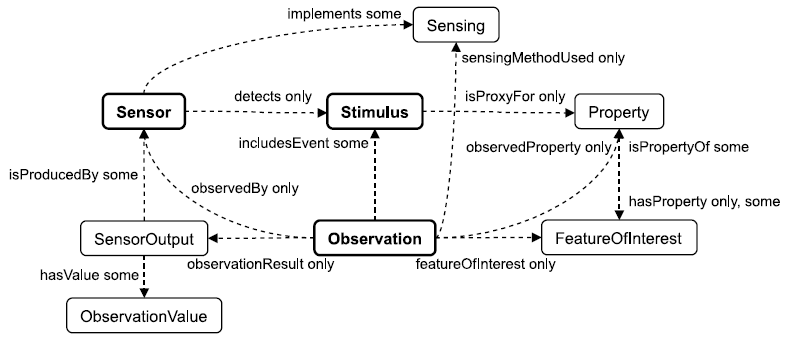
\includegraphics[width=1\linewidth]{figs/sens_stim_obs.png}
	\caption{The stimulus–sensor–observation pattern \cite[p. 28]{SSW:SSN_incubatorGroup}}
	\label{fig:sens-stim-obs}
\end{figure}

\subsection{Observation capability metadata model} 
\cite{SW:Hu} have reviewed a number of metadata models (including \ac{sensorml} and \ac{ssno}) for the use of earth observation (including remote sensing). They argue that all of the current metadata models are not sufficient for sensor data discovery. This conclusion is based on an evaluation of six criteria. Three steps were identified in the process of obtaining relevant sensor data for earth observation, which have been used to derive criteria for their evaluation framework. These steps are sensor filtration, sensor optimisation and sensor dispatch. The filtration of sensors should result in a set of sensors that meets the requirements of the application: It should measure the right phenomenon, be active, be inside the spatial and temporal range, and have a certain sample interval. In sensor optimisation the selected sensors should be combined to complement or enhance each other. To do this, the observation quality, coverage and application is relevant. In the last step -- sensor dispatch -- the data should be retrieved, stored and transmitted. In every evaluated model the same sensors can be described in different ways or only partially, which affects the outcome of the sensor dispatch. 

Therefore, a metadata model is proposed that \enquote{reuses and extends the existing sensor observation-related metadata standards} \cite[p. 10546]{SW:Hu}. It is composed of five modules: observation breadth, observation depth, observation frequency, observation quality and observation data. They should be derived from metadata elements described using the Dublin Core metadata element set. These five modules can then be formalised following the \ac{sensorml} schema which can be queried by users via a `Unified Sensor Capability Description Model-based Engine'. 

\subsection{Om-lite \& sam-lite ontologies}
\cite{SSW:Cox4} has been working on new semantic ontologies based on \ac{om}. Previous efforts, such as the \ac{ssno} have been using pre-existing ontologies and frameworks. However, there are already many linked data ontologies that could be useful for describing observation metadata, such as space and time concepts. Also, the \ac{ssno} does not take sampling features into account. Therefore, \cite{SSW:Cox4} proposes two new ontologies: \ac{owl} for observations or om-lite \citep{SSW:Cox3}, which defines the concepts from \ac{om} regarding observations and \ac{owl} for sampling features or sam-lite, which defines the sampling feature concepts \citep{SSW:Cox2}. A mapping of the \ac{ssno} to om-lite is also provided.

\cite{SSW:Cox4} describes how the PROV ontology \citep{LD:PROV} can be directly used inside om-lite. The PROV ontology is \enquote{concerned with the production and transformation of Entities through time-bounded Activities, under the influence or control of Agents} \cite[p. 12]{SSW:Cox4}. This is a very convenient ontology for modelling real world entities, such as sensors, observation processes and sampling processes. Many other ontologies could be implemented in combination with om-lite and sam-lite, depending on the kind of observations that are being modelled and the data publisher's preference. 

\section{Sensor data aggregation}
Sensor data aggregation can be performed for two purposes: To reduce the energy constraint of sensor networks \citep{SW:Korteweg} or to sample a feature-of-interest in space and/or time \citep{SDI:INSPIRE2}. Sampling is performed when a feature-of-interest is not accessible, in which case \enquote{observations are made on a subset of the complete feature, with the intention that the sample represents the whole} \citep{SSW:Cox3}. \cite{SSW:Stasch3} proposes a \ac{wps} that retrieves sensor data from a \ac{sos} service in order to aggregate it based on features-of-interest. The approach by \cite{SSW:Stasch} is similar, but takes sensor data as input that is already published on the semantic web.

\cite{SW:Ganesan} stresses that spatio-temporal irregularities are fundamental to sensor networks. Irregular sampling can have a potentially large influence on the accuracy of the aggregated outcome. For example, averaging sensor data from a feature-of-interest that is being sampled densely in some parts and more sparsely in other parts could lead to inaccurate results. To counter this the values of the densely sampled area should have a lower weight than the values from the sparsely sampled area. The same holds true for temporal irregularities \citep{SW:Ganesan}. Also, \cite{SSW:Stasch4} argue that in order for automatic aggregation to work there needs to be semantics on which kind of aggregation methods are appropriate for a specific kind of sensor data. Not all kinds of aggregation are meaningful (e.g. taking the sum of temperature values). This requires a formalisation of expert knowledge which they call semantic reference systems. 




